\documentclass[a4paper]{article}

\usepackage[english]{babel}
\usepackage[utf8x]{inputenc}
\usepackage{amsmath}
\usepackage{graphicx}
\usepackage[colorinlistoftodos]{todonotes}

\title{CS5785 Lecture 20 Scribe Notes}
\author{Prof. Nathan Kallus, Cornell Tech \\Scribe: TBD}
\date{Nov.\ 9, 2017 (Under construction)}


\begin{document}
\maketitle

\section{Convolutional Neural Networks (ConvNets)}

The example of the training cases from ZIP code data (HTF Fig.~11.9) is a character recognition task, which captured the attention of the machine learning and neural network community for many years, and has remained a benchmark problem in the field. However, the neural networks we saw in the last lecture are ill-suited to this problem: pixel representation of images change disproportionately under small affine transfer (rotation, translation, etc.). Motivated by this, in the late 1980s Yann LeCun (then at Bell Labs, now at Facebook \& NYU) pioneered a variant of neural networks to overcome this problem.\\

\section{Review Net-1 through Net-5}

\begin{figure}[h]
\centering
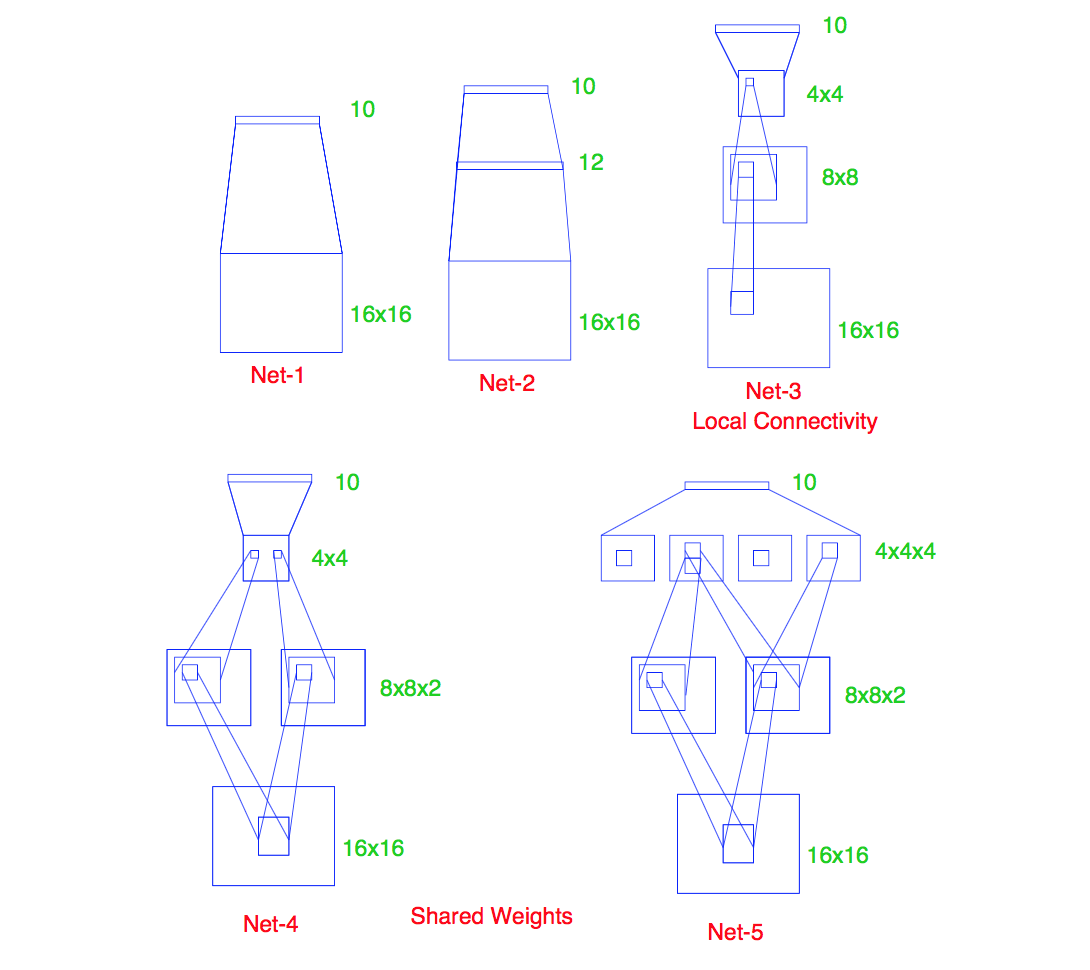
\includegraphics[width=0.7\textwidth]{Architecture_of_the_five_networks}
\caption{Architecture of the five networks used in the ZIP code example [HTF Figure 11.10]}
\end{figure}

\textbf{Net-1}: 256 inputs, 10 outputs for predicted value $f_{k}(\underline{x}), k=0, ..., 9$. All have sigmoidal output units, all fit with sum-of-squares error function. Net-1 has no hidden layer, and is equivalent to  multinomial logistic regression generalized to n (10 here) classes. Net-1 is prone to overfitting as evident from  Figure \ref{fig:test_performance_curves} (observe that, performance on test data increases and falls with more training epochs).\\

\textbf{Net-2}: Net-2 has 12 hidden units and it is \textit{fully connected}. Here, fully connected means each of the 256 pixels in input image is connected to each hidden node and each hidden node is connected to output node). Note that the training set error approaches $0\%$ in all these cases since we have many more parameters than training observations. \\

\begin{figure}[h]
\label{fig:test_performance_curves}
\centering
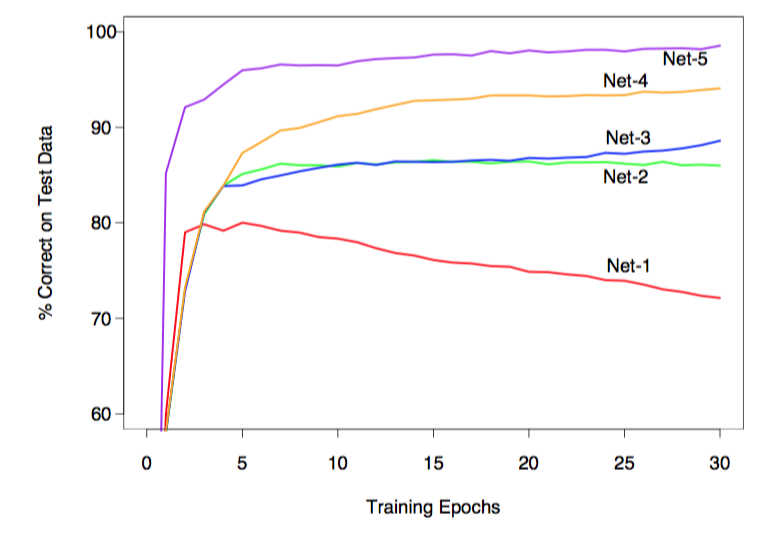
\includegraphics[width=0.9\textwidth]{Test-Performance-Curves}
\caption{Test performance curves [HTF Figure 11.11]}
\end{figure}


\textbf{Net-3}: Things get more interesting with Net-3 which uses local connectivity. Instead of fully connected, each hidden unit is connected only to a small patch of units in the layer below. In first hidden layer ($8\times 8$ array), each unit takes input from a $3\times 3$ patch in input layer. Their receptive fields ``stride'' of 2 pixels in input layer corresponds to an overlap of one row or column, and hence are two pixels apart. Second hidden layer ($4\times 4$ array) takes input from $5\times 5$ receptive field. Outside this local connection regions, weights are tied to zero. Local connectivity makes each unit responsible for extracting "local features" from the layer below. Figure \ref{table11-11} shows how links and weights influence the accuracy, where Net-3 has fewer links and weights but lower misclassification rate.\\


\begin{figure}[h]
\label{table11-11}
\centering
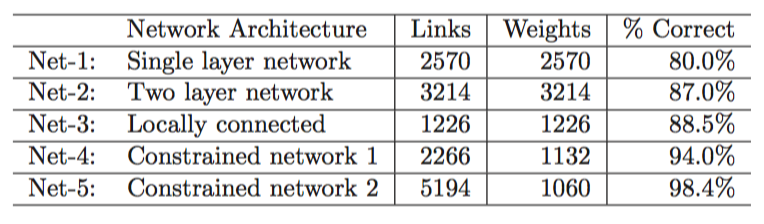
\includegraphics[width=0.8\textwidth]{Test_set_performance_of_five_different_neural_networks_on_a_hand-_written_digit_classification_example}
\caption{Test set performance of five different neural networks on a hand- written digit classification example (LeCun, 1989). [HTF Table 11.1]}
\end{figure}


\begin{figure}[h]
\centering
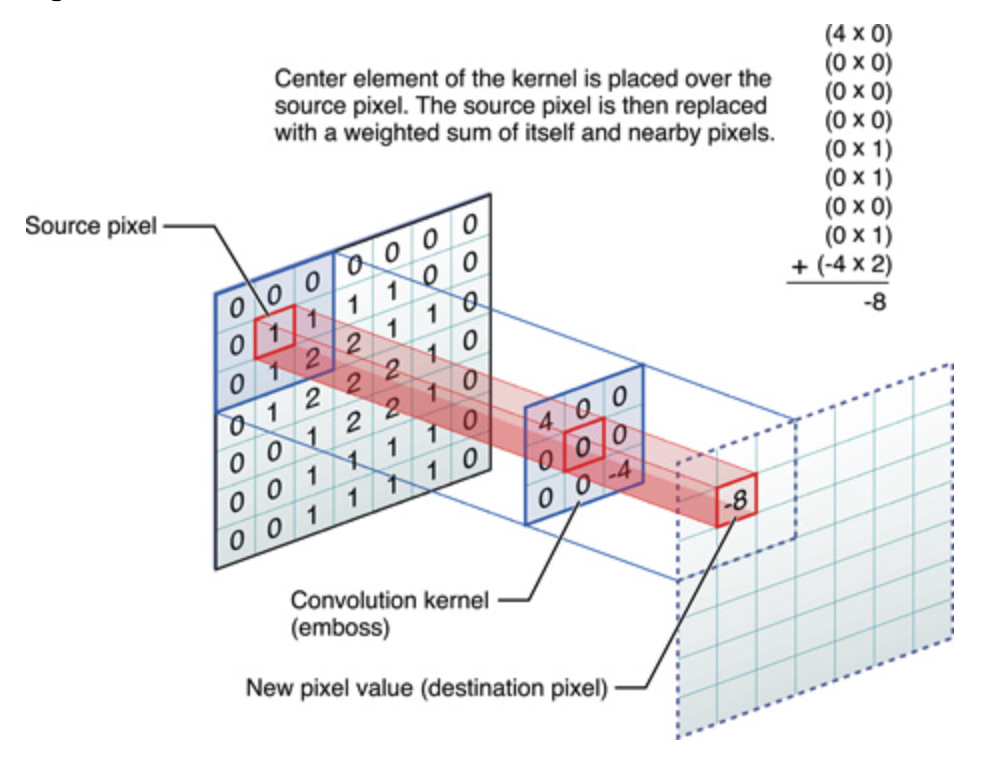
\includegraphics[width=0.8\textwidth]{Kernel_convolution}
\caption{Kernel convolution}
\end{figure}

\textbf{Net-4}: Net-4 has two hidden layers, and uses locally connectivity with weight sharing. Net-4’s first hidden layer is similar to that of Net-3; it has two 8×8 arrays instead of one, each unit taking input from a 3×3 patch. However, each of the units in the same 8×8 feature map share the same set of nine weights. These nine weights are equivalent to convolution kernels. 
\\The second hidden layer of Net-4 has no weights sharing, same as Net-3. From Figure 3 we see that Net-4 has more links but fewer weights than Net-3, but performs better.\\ \\
\textbf{Net-5}: Net-5 has two local-connected hidden layers and two levels of weight sharing. It has four 4 × 4 feature maps in the second hidden layer, where each unit is connected to a 5 × 5 local patch in the layer below. Weights are shared in each of these feature maps. The clever design of network Net-5 is the result of many years of experimentation, using domain knowledge of handwritten digits into their design. This also shows that neural networks are not a fully automatic tool, as they are sometimes advertised.\\


\end{document}
